\documentclass[a4paper,11pt,twoside]{article}
%\documentclass[a4paper,11pt,twoside,se]{article}

\usepackage{UmUStudentReport}
\usepackage{verbatim}   % Multi-line comments using \begin{comment}
\usepackage{courier}    % Nicer fonts are used. (not necessary)
\usepackage{pslatex}    % Also nicer fonts. (not necessary)
\usepackage[pdftex]{graphicx}   % allows including pdf figures
\usepackage{listings}
\usepackage{pgf-umlcd}
%\usepackage{lmodern}   % Optional fonts. (not necessary)
%\usepackage{tabularx}
%\usepackage{microtype} % Provides some typographic improvements over default settings
%\usepackage{placeins}  % For aligning images with \FloatBarrier
%\usepackage{booktabs}  % For nice-looking tables
%\usepackage{titlesec}  % More granular control of sections.

% DOCUMENT INFO
% =============
\department{Department of Computing Science}
\coursename{Object-Oriented Programming Methodology 7.5 p}
\coursecode{5DV133}
\title{OU1 Clock}
\author{Lorenz Gerber ({\tt{dv15lgr@cs.umu.se}} {\tt{lozger03@student.umu.se}})}
\date{2016-04-07}
%\revisiondate{2016-01-18}
\instructor{Anders Broberg / Niklas Fries / Adam Dahlgren / Jonathan
  Westin / Erik Moström / Alexander Sutherland}


% DOCUMENT SETTINGS
% =================
\bibliographystyle{plain}
%\bibliographystyle{ieee}
\pagestyle{fancy}
\raggedbottom
\setcounter{secnumdepth}{2}
\setcounter{tocdepth}{2}
%\graphicspath{{images/}}   %Path for images

\usepackage{float}
\floatstyle{ruled}
\newfloat{listing}{thp}{lop}
\floatname{listing}{Listing}



% DEFINES
% =======
%\newcommand{\mycommand}{<latex code>}

% DOCUMENT
% ========
\begin{document}
\lstset{language=C}
\maketitle
\thispagestyle{empty}
\newpage
%\tableofcontents
%\thispagestyle{empty}
%\newpage

\clearpage
\pagenumbering{arabic}

\section{Introduction} 
Aim of this laboration was to implement a model of a digital clock and
an alarm clock in the object oriented language Java. The class design
was mostly defined in the specifications \cite{clock}. After
implementing \textit{Clock} and \textit{Alarm} classes, a
\textit{main} method had to be written to provide test cases for the
implemented classes. Additionally, it was also recommended to write
JUnit tests for all classes.

\section{Usage Instructions}
The files provided in an zip archieve: \textit{ClockApp.java,
  Clock.java, ClockTest.java, NumberDisplay.java,
  NumberDisplayTest.java, Alarm.java, AlarmTest.java}. To build from
the command line, \textit{javac ClockApp.java} is invoked. To run the
program \textit{java ClockApp}. The main program \textit{ClockApp}
does not take any input. On execution it writes output to the
screen. The implications of the printout will be described further in
the section \textit{testing}. 

\section{System Description}
First Class Responsibility Collaborators \textit{CRC} Tables were
drawn for all classes (\textit{Table \ref{tab:crcclock},
\ref{tab:crcnumberdisplay}, \ref{tab:crcalarm}}). The specification
did not demand an actual running clock, just a model that would have
all the functionality. Hence the advancement of the time had to be
done manually in the main program.

The UML class diagrams shown here are basically the same as those
given in the assignment (\textit{Figure \ref{fig:umlclass}}). However,
the \textit{Alarm} class was added. The \textit{Clock} aggregates two
\textit{NumberDisplays}. The \textit{Alarm} inherits this from the
\textit{Clock} but aggregates two additional \textit{NumberDisplays}
to keep track of the alarm time. This could also have been solved as
primitive datatype properties in the \textit{Alarm} class. Here it was
however decided to reuse the components, and keep it flexible if
further functionality should be implemented later on.



\begin{table}[!h]
\centering
\caption{\textit{`Class Responsibility Collaborators' tables for Clock}}
\label{tab:crcclock}
\begin{tabular}{l|l}
Class: Clock              &                        \\ \hline
\textbf{Responsibilities} & \textbf{Collaborators} \\
knows hours               & NumberDisplay          \\
knows minutes             &                        \\
                          &                        \\
show time                 &                        \\
set time                  &                        \\
advance minutes           &                       
\end{tabular}
\end{table}

\begin{table}[h]
\centering
\caption{\textit{`Class Responsibility Collaborators' tables for NumberDisplay}}
\label{tab:crcnumberdisplay}
\begin{tabular}{l|l}
Class: Number Display     &                        \\ \hline
\textbf{Responsibilities} & \textbf{Collaborators} \\
knows minLimit            & Clock                  \\
knows maxLimit            &                        \\
knows current value       &                        \\
                          &                        \\
show value                &                        \\
advance value             &                        \\
check if wrapped around   &                       
\end{tabular}
\end{table}

\begin{table}[h]
\centering
\caption{\textit{`Class Responsibility Collaborators' tables for
    Alarm.}}
\label{tab:crcalarm}
\begin{tabular}{l|l}
Class: Alarm - extends Clock &                        \\ \hline
\textbf{Responsibilities} & \textbf{Collaborators} \\
knows alarm hours         & NumberDisplay          \\
knows alarm minutes       &                        \\
know if it is alarm       &                        \\
                          &                        \\
set alarm                 &                        \\
switch on / off alarm     &                        \\
alarm!                    &                       
\end{tabular}
\end{table}

\begin{figure}
  \centering
  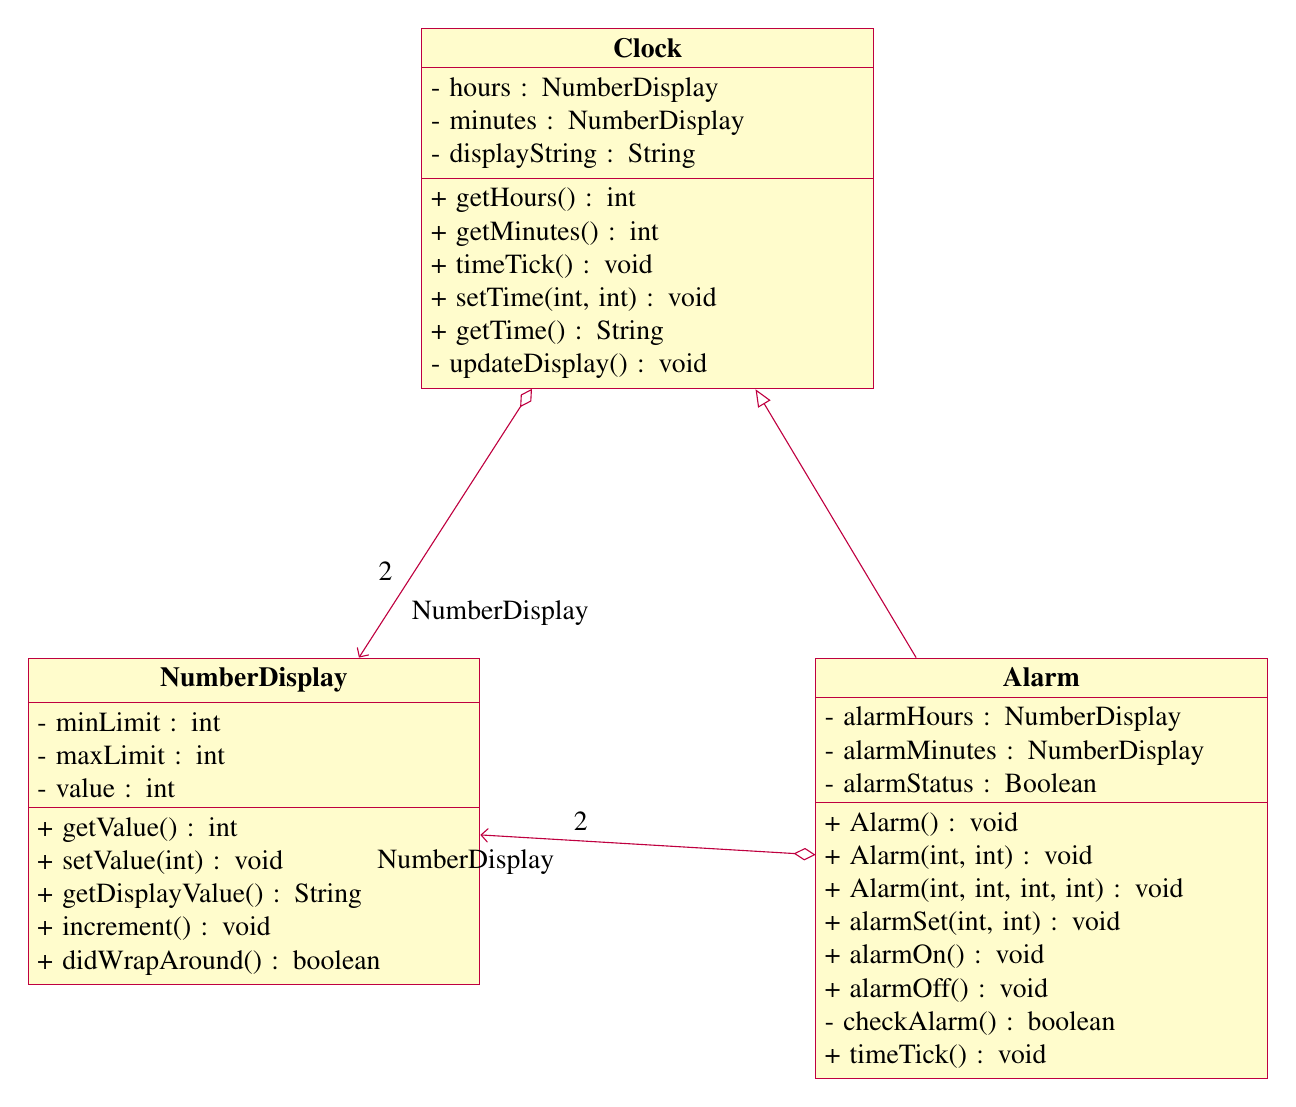
\begin{tikzpicture}
    \begin{class}[text width = 5.5cm]{Clock}{0,0}
      \attribute{- hours : NumberDisplay}
      \attribute{- minutes : NumberDisplay}
      \attribute{- displayString : String}

      \operation{+ getHours() : int}
      \operation{+ getMinutes() : int}
      \operation{+ timeTick() : void}
      \operation{+ setTime(int, int) : void} 
      \operation{+ getTime() : String}
      \operation{- updateDisplay() : void}
    \end{class}
    
    \begin{class}[text width = 5.5cm]{Alarm}{5,-8}
      \inherit{Clock}

      \attribute{- alarmHours : NumberDisplay}
      \attribute{- alarmMinutes : NumberDisplay}
      \attribute{- alarmStatus : Boolean}

      \operation{+ Alarm() : void}
      \operation{+ Alarm(int, int) : void}
      \operation{+ Alarm(int, int, int, int) : void}
      \operation{+ alarmSet(int, int) : void}
      \operation{+ alarmOn() : void}
      \operation{+ alarmOff() : void}
      \operation{- checkAlarm() : boolean}
      \operation{+ timeTick() : void}
    \end{class}


    \begin{class}[text width = 5.5cm]{NumberDisplay}{-5, -8}
      \attribute{- minLimit : int}
      \attribute{- maxLimit : int}
      \attribute{- value : int}

      \operation{+ getValue() : int}
      \operation{+ setValue(int) : void}
      \operation{+ getDisplayValue() : String}
      \operation{+ increment() : void}
      \operation{+ didWrapAround() : boolean}
    \end{class}
    \aggregation{Clock}{NumberDisplay}{2}{NumberDisplay}
    \aggregation{Alarm}{NumberDisplay}{2}{NumberDisplay}
  \end{tikzpicture}
  \caption{\textit{Class diagrams of Clock and NumberDisplay.}}
  \label{fig:umlclass}  
\end{figure}




\subsection{Checking for wrap around}
In the specifications it was given that \textit{didWrapAround} is a
method. There are different ways how this check can be
implemented. The most simplistic is to check whether minutes is 0 and
deduce from it that it wrapped around on the last
\textit{minutes.increment}. Another way would be to add a boolean
property variable that can be set to true when actual wrapping
happens.

\subsection{Checking for Alarm condition}
In the specifications it was given that the check for alarm should
happen in the \textit{timeTick} method. Hence, setting time or alarm
to the same time will not produce an alarm event as the alarm
condition will be checked after the \textit{minutes.increment} in the
\textit{timeTick} method. Implementing the feature to check for alarm
condition after both setting time or alarm time can be implemented in
many ways. The determining factor is that alarm check happens in the
\textit{timeTick} method. Hence one way could be to decrease the
minutes counter one minute and then call for the \textit{timeTick}
method that would also check for alarm condition in the actual set
time. However, this implementation creates a complicated edge case for
the value 0. When setting time to 0, it will be decreased to -1 to
advance then to 1. This will however detect wrap around condition and
advance the hour by one. Hence, to implement this feature, it could
make sense to store wrap around condition when it actually happens in
a seaparate boolean property. 

 
\section{Testing}
Testing was conducted in the main program. Additionally, JUnit4 test
files were written and tested. The JUnit test cases check wheter the
constructors works and for the \textit{IllegalArgumentException}. More
detailed logical testing was done in the main program which 
included nine usecases which were all run on the \textit{Alarm}
class. For the sake of simplicity, now logic was built in to check for
passed or not passed. However, after reading the specification of the
classes, the expected result should be obvious.

First a new object was instantiated. Then the default time of the
clock modul is written to screen. Next, alarm time is set to clock
time. Due to the specific implementation of the program, no alarm is
expected. The opposite case is tested next where the clock is set to
an activated alarm time. Also here, due to the specific
implementation, no alarm event happens. Then incrementing the time
through a full cycle with activated alarm should create an alarm
event. Next, the same situation is tested with alarm deactivated.
Exception handling for out of range input was implemented in all
classes. Here exception handling for such a case is tested next.
Finally, two edge cases are tested. First incrementing from time 00:00
to 00:01 and then from 23:59 to 00:00. 



\addcontentsline{toc}{section}{\refname}
\bibliography{references}

\end{document}
